	\documentclass[10pt,twocolumn,letterpaper]{article}

\usepackage{cvpr}
\usepackage{times}
\usepackage{epsfig}
\usepackage{graphicx}
\usepackage{amsmath}
\usepackage{amssymb}
% Include other packages here, before hyperref.
%\usepackage{natbib}
% If you comment hyperref and then uncomment it, you should delete
% egpaper.aux before re-running latex.  (Or just hit 'q' on the first latex
% run, let it finish, and you should be clear).
\usepackage[pagebackref=true,breaklinks=true,letterpaper=true,colorlinks,bookmarks=false]{hyperref}
\cvprfinalcopy % *** Uncomment this line for the final submission

\def\cvprPaperID{****} % *** Enter the CVPR Paper ID here
\def\httilde{\mbox{\tt\raisebox{-.5ex}{\symbol{126}}}}

% Pages are numbered in submission mode, and unnumbered in camera-ready
%\ifcvprfinal\pagestyle{empty}\fi

\graphicspath{{../figs/}}


\begin{document}

%%%%%%%%% TITLE
\title{Image Completion: Milestone}

\author{Debora Sujono, Yue Tang \& Grace Yoo \\ 
University of Massachusetts Amherst \\ 
College of Information \& Computer Sciences \\
{\tt\small \{dsujono, gyoo, ytang\}@cs.umass.edu} \\
}

\maketitle
%\thispagestyle{empty}

%%%%%%%%% BODY TEXT
\section{Introduction}
%Introduction: this section introduces your problem, and the overall plan for approaching your problem
Image completion, which is also called content-aware fill or inpainting, is a generative technique that can be used to fill missing areas of an image. The desired result is an image that a human would perceive as normal. These techniques are often implemented in photo-editing software to mend corrupted images.

\par We can conceptualize a photograph as a low-dimensional sample from a high-dimensional distribution, the original scene. The problem can be framed as learning these high-dimensional distributions such that we can generate a sample that approximates missing pixels. Contextual information from incomplete images, such as the values of pixels neighboring the missing content, can help inform the generative model. On a higher level, perceptual information, such as understanding what a normal image looks like, is necessary to generate images that humans will believe. %% cite blog?

\par We will build a generative model to create samples with which to fill in missing areas of images. A generative model typically takes some hidden parameters and then randomly generates values from a joint probability distribution that covers labeled observations. In the context of our problem, a generative model will learn the hidden parameters that determine normal image structures and simulate values for all pixels of an image.

\section{Problem statement}
%Problem statement: Describe your problem precisely specifying the dataset to be used, expected results and evaluation
Given an image with a square region of missing pixels, our goal is to fill in the missing pixels to create a cohesive image. We will use the CIFAR-10 dataset, which consists of $60,000$ images evenly distributed into 10 classes (airplane, automobile, bird, cat, deer, dog, frog, horse, ship, truck). Each $32$ x $32$ x $3$ pixel image is represented by the RGB color model. We will remove a square region of each image, and consider the original image to be the original distribution of $32$ x $32$ x $3 = 3,072$ dimensions. 

\par As our baseline, we will implement a convolutional neural net (CNN) with mean squared error (MSE) loss between incomplete and original images, to perform regression on the intensities of the missing pixels. From here, we will each investigate different generative modeling methods to improve the baseline score using the same evaluation.

\par After experimentation, we will optimize one or two models that we find most promising. We will use Root Mean Squared Error (RMSE) to compare models. The RMSE will give us an idea of how well our generated images compare to the originals; however, the problem is to generate any plausible images, so we will also randomly sample images for human judgment. We will ask judges to rate an image as "plausible" or "not plausible", and determine which models generate the most believable images. 

This is what our incomplete images look like after we mask part of it:

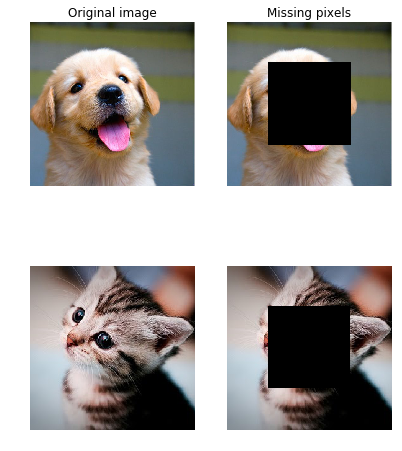
\includegraphics[width=1.0\linewidth]{img_sample.png}

Once we create a model that we can generate samples from, we'll use the model to create filled-in images $\hat{y}$.

Given the set of generated images $\hat{y}$. and corresponding original images $y$, we want to learn network parameters  $ \theta = [W_1, b_1, W_2, b_2, W_3, b_3]$ that minimize the MSE between generated and original images (or between incomplete and original images for the baseline case). 

\section{Technical Approach}

%Technical Approach: Describe the methods you intend to apply to solve the given problem
Training a generative model can easily become intractable; we not only have to simulate high dimensional distributions, but also apply some kind of inference method. In the following sections, we will outline the probabilistic underpinnings of the different training methods that we will implement. 

\subsection{Generative Adversarial Networks}
Generative Adversarial Networks (GANs) train two networks simultaneously; a discriminator $D(x)$ that says whether an image $x$ is an original or generated, and a generator that produces input $x$ for the discriminator. The generator network takes a parameter $Z$, a random sample from a distribution (such as Gaussian), and generates image $G(Z)$.

\par The discriminator outputs a scalar $D(x)$ for each image $x$; let's say that for an original image, $D(x)$ is low, while for generated images $D(x) = D(G(Z))$ is high. The discriminator's objective is simply to adjust parameters to score images accurately; in other words, to maximize $D(x)$.

The generator, on the other hand, wants to produce an image $G(Z)$ such that the discriminator thinks it's an original, so it wants to minimize $D(G(Z))$. In this sense, we can describe the generator and discriminator as two players in a minimax game \cite{GAN}

After the generator is trained, we can use it to create $\hat{y}$. 

%We expect that images generated by $G(Z)$ will be rather noisy.

\subsection{Deep Convolutional Generative Adversarial Networks}
Deep Convolutional Generative Adversarial Networks (DCGAN) aim to scale GANs by using CNNs and adding some extra constraints to help stabilize training. Here are the guidelines outlined by Radford, Metz, and Chintala \cite{DCGAN}:
\begin{itemize}
\item Replace pooling layers with
\subitem fractional-strided convolutions in the generator
\subitem strided convolutions in the discriminator
\item Use batchnorm in both networks
\item If the network is quite deep, remove any fully connected hidden layers
\item Activation functions
\subitem Tanh for the generator output layer
\subitem ReLU in the rest of generator layers 
\subitem leaky ReLU in all discriminator layers
\end{itemize}

For both GAN and DCGAN implementations, we will start with an existing one from this list: \\
 \url{https://bamos.github.io/2016/08/09/deep-completion/#existing-gan-and-dcgan-implementations}.

\subsection{Pixel Recurrent Neural Networks}
Recurrent Neural Networks (RNNs) solve the problem of efficiently modeling the joint distribution of pixels in the image by treating it as a product of conditional distributions. This converts the problem into a sequence problem, and the task becomes to predict the next pixel given the previously generated ones \cite{pixelRNN}. 

Let $p(x)$ be the generated distribution for image $x$ with dimensions [$n$ x $n$], represented as a row of length $n^2$. We approximate $p(x)$ by: \\
$p(x) = \prod_{i=1}^{n^2} p(x_i | x_1, ... , x_{i-1} )$

Pixel CNN is like Pixel RNN, but uses convolutional layers to cut computational costs \cite{pixelCNN}. We will use the TensorFlow implementations for Pixel RNN and Pixel CNN. \url{https://github.com/carpedm20/pixel-rnn-tensorflow}

%\subsection{Image completion with perceptual and contextual losses}

\section{Preliminary Results}
%Intermediate/Preliminary Results: State and evaluate your results upto the milestone
We have implemented a 3-layer CNN with regression using the following architecture: 
%$Convolutional \rightarrow ReLU \rightarrow 2x2 Max pooling \rightarrow affine \rightarrow ReLU \rightarrow affine \rightarrow MSE$

\begin{itemize}
\item Input: [32 x 32 x 3] raw pixel values
\item Convolutional layer with [7 x 7] filter
%\subitem results [32 x 32 x 7]
\item ReLU activation
\item Pooling layer [2 x 2]
%: results [16 x 16 x 7]
\item Affine
\item ReLU activation
\item Affine
\item Output: sum previous layer, use RMSE loss function
\end{itemize}

This is not the final architecture we will use, we just decided to start with the architecture from Assignment 2 while we debug these first steps. 

We then trained the network for 1 epoch and achieved training RMSE of 120.323 and validation RMSE of 153.462. Our network is currently overfit, and since the values of the data range from 0.0 - 255.0, these RMSE values are quite high. We expect high RMSE because this is just the baseline network, but we are currently checking to make sure there aren't other issues causing such a high RMSE.

\begin{thebibliography}{1}
\bibitem{pixelRNN} Conditional Image Generation with PixelCNN Decoders \url{https://arxiv.org/pdf/1606.05328v2.pdf}
\bibitem{pixelRNN} Pixel Recurrent Neural Networks \url{https://arxiv.org/pdf/1601.06759v3}
\bibitem{GAN} Generative Adversarial Nets \url{http://papers.nips.cc/paper/5423-generative-adversarial-nets.pdf}
\bibitem{DCGAN} Unsupervised Representation Learning with Deep Convolutional Generative Adversarial Networks \url{https://arxiv.org/pdf/1511.06434v2}
\bibitem{inpaint} Semantic Image Inpainting with Perceptual and Contextual Losses \url{https://arxiv.org/pdf/1607.07539v2.pdf}
\end{thebibliography}

%
\bibliographystyle{unsrtnat}
\bibliography{milestone}




\end{document}
